% Preamble:
% \usepackage{tikz}
% \usepackage{subcaption}

\begin{figure}[ht]
\centering

\begin{subfigure}[t]{0.32\textwidth}
\centering
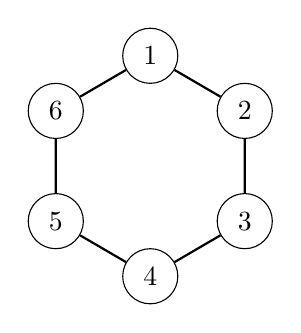
\begin{tikzpicture}[
  v/.style={circle, draw, minimum size=7mm},
  e/.style={thick}
]
\node[v] (1) at (0,1.4) {1};
\node[v] (2) at (1.2,0.7) {2};
\node[v] (3) at (1.2,-0.7) {3};
\node[v] (4) at (0,-1.4) {4};
\node[v] (5) at (-1.2,-0.7) {5};
\node[v] (6) at (-1.2,0.7) {6};
\draw[e] (1)--(2)--(3)--(4)--(5)--(6)--(1);
\end{tikzpicture}
\caption{$C_6$ (2-regular)}
\end{subfigure}
\hfill
\begin{subfigure}[t]{0.32\textwidth}
\centering
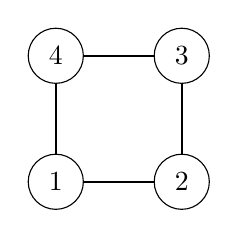
\begin{tikzpicture}[
  v/.style={circle, draw, minimum size=7mm},
  e/.style={thick}
]
\node[v] (1) at (0,0) {1};
\node[v] (2) at (1.6,0) {2};
\node[v] (3) at (1.6,1.6) {3};
\node[v] (4) at (0,1.6) {4};
\draw[e] (1)--(2)--(3)--(4)--(1);
\end{tikzpicture}
\caption{$C_4$ (2-regular)}
\end{subfigure}
\hfill
\begin{subfigure}[t]{0.32\textwidth}
\centering
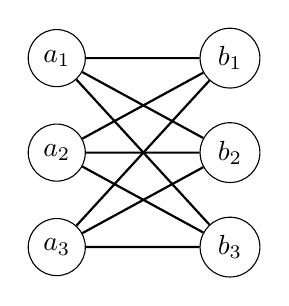
\begin{tikzpicture}[
  v/.style={circle, draw, minimum size=7mm},
  e/.style={thick}
]
\node[v] (a1) at (0, 1.2) {$a_1$};
\node[v] (a2) at (0, 0.0) {$a_2$};
\node[v] (a3) at (0,-1.2) {$a_3$};

\node[v] (b1) at (2.2, 1.2) {$b_1$};
\node[v] (b2) at (2.2, 0.0) {$b_2$};
\node[v] (b3) at (2.2,-1.2) {$b_3$};

\draw[e] (a1)--(b1) (a1)--(b2) (a1)--(b3);
\draw[e] (a2)--(b1) (a2)--(b2) (a2)--(b3);
\draw[e] (a3)--(b1) (a3)--(b2) (a3)--(b3);
\end{tikzpicture}
\caption{$K_{3,3}$ (3-regular)}
\end{subfigure}

\caption{Examples of regular graphs: $C_6$ and $C_4$ are 2-regular; $K_{3,3}$ is 3-regular.}
\label{fig:regular-examples}
\end{figure}
